\section{ITSA-58-2 道路修補}
\centerline{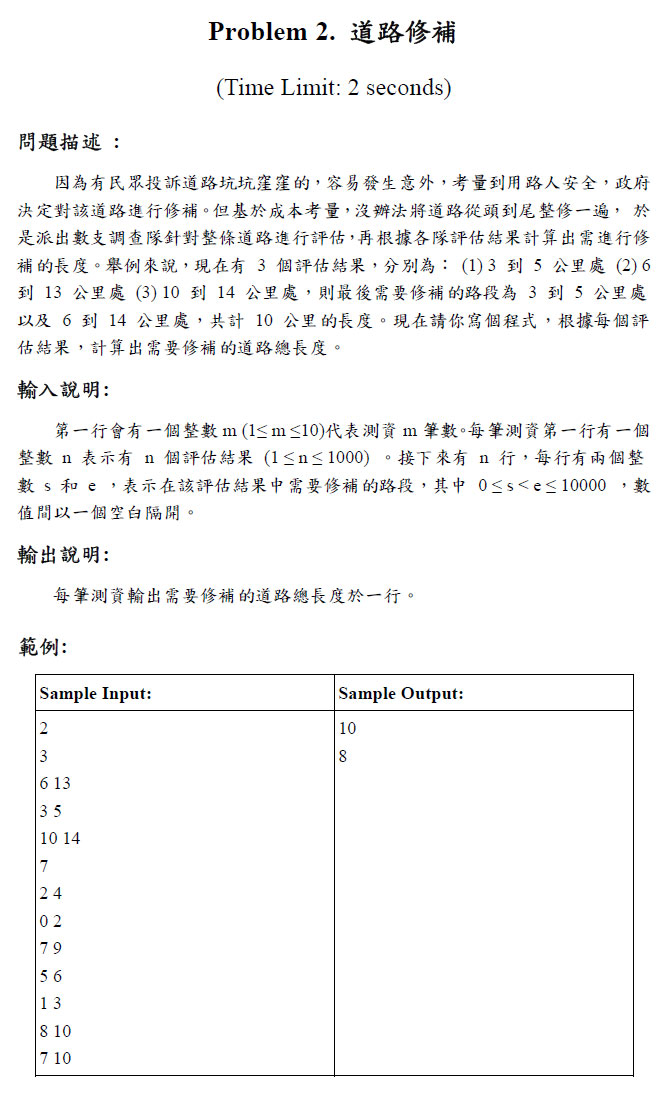
\includegraphics[height=.95\textheight]{../solutions/fig/58ITSA2}}

\subsection{解題思惟}
\begin{enumerate}
	\item m個case的情理方式,同第1題。每個case又有n個評估結果,這個處理方式也相同。
	\item 每一個評估結果,都會輸入s和e,等於是一個線段。最後要求的,其是就是所有n個線段聯集的長度。要怎麼處理聯集的長度呢?
	\item 題目有限制最大的e值不超過10000,那我們可以用一個很簡單的方式來處理,就是直接記錄每一個單位長度i到i+1是否被包含在聯集裡,這樣的話,最多也只有10000個單位線段,那我們可以設一個10000個元素以上的陣列lend,如果線段i到i+1被包含在聯集裡,我們就設lend[i]=1,如果不包含在聯集裡,就設lend[i]=0。最後要求聯集的長度,就把陣列所有元素加總就可以了。
	\item 換一個角度思考,我們可以先把陣列所有元素都設為0,那當我們讀入一個線段[s,e]的時候,直接把lend[s]一直到lend[e-1]全部設為1就可以了。
\end{enumerate}

\subsection{程式碼}
\begin{cppcode}
#include <iostream>

using namespace std;

int main()
{
	int kase, n, s, e, lend[10000];
	while (kase--) {
		for (int i=0; i<10000; i++) lend[i]=0;
		cin >> n;
		while (n--) {
			cin >> s >> e;
			for (int i=s; i<e; i++) lend[i]=1;
		}
		int sum = 0;
		for (int i=0; i<10000; i++) sum+=lend[i];
		cout << sum << endl;
	}
	return 0;
}	
\end{cppcode}